\section{你的第三章标题}

\begin{figure}[H]
	\centering
	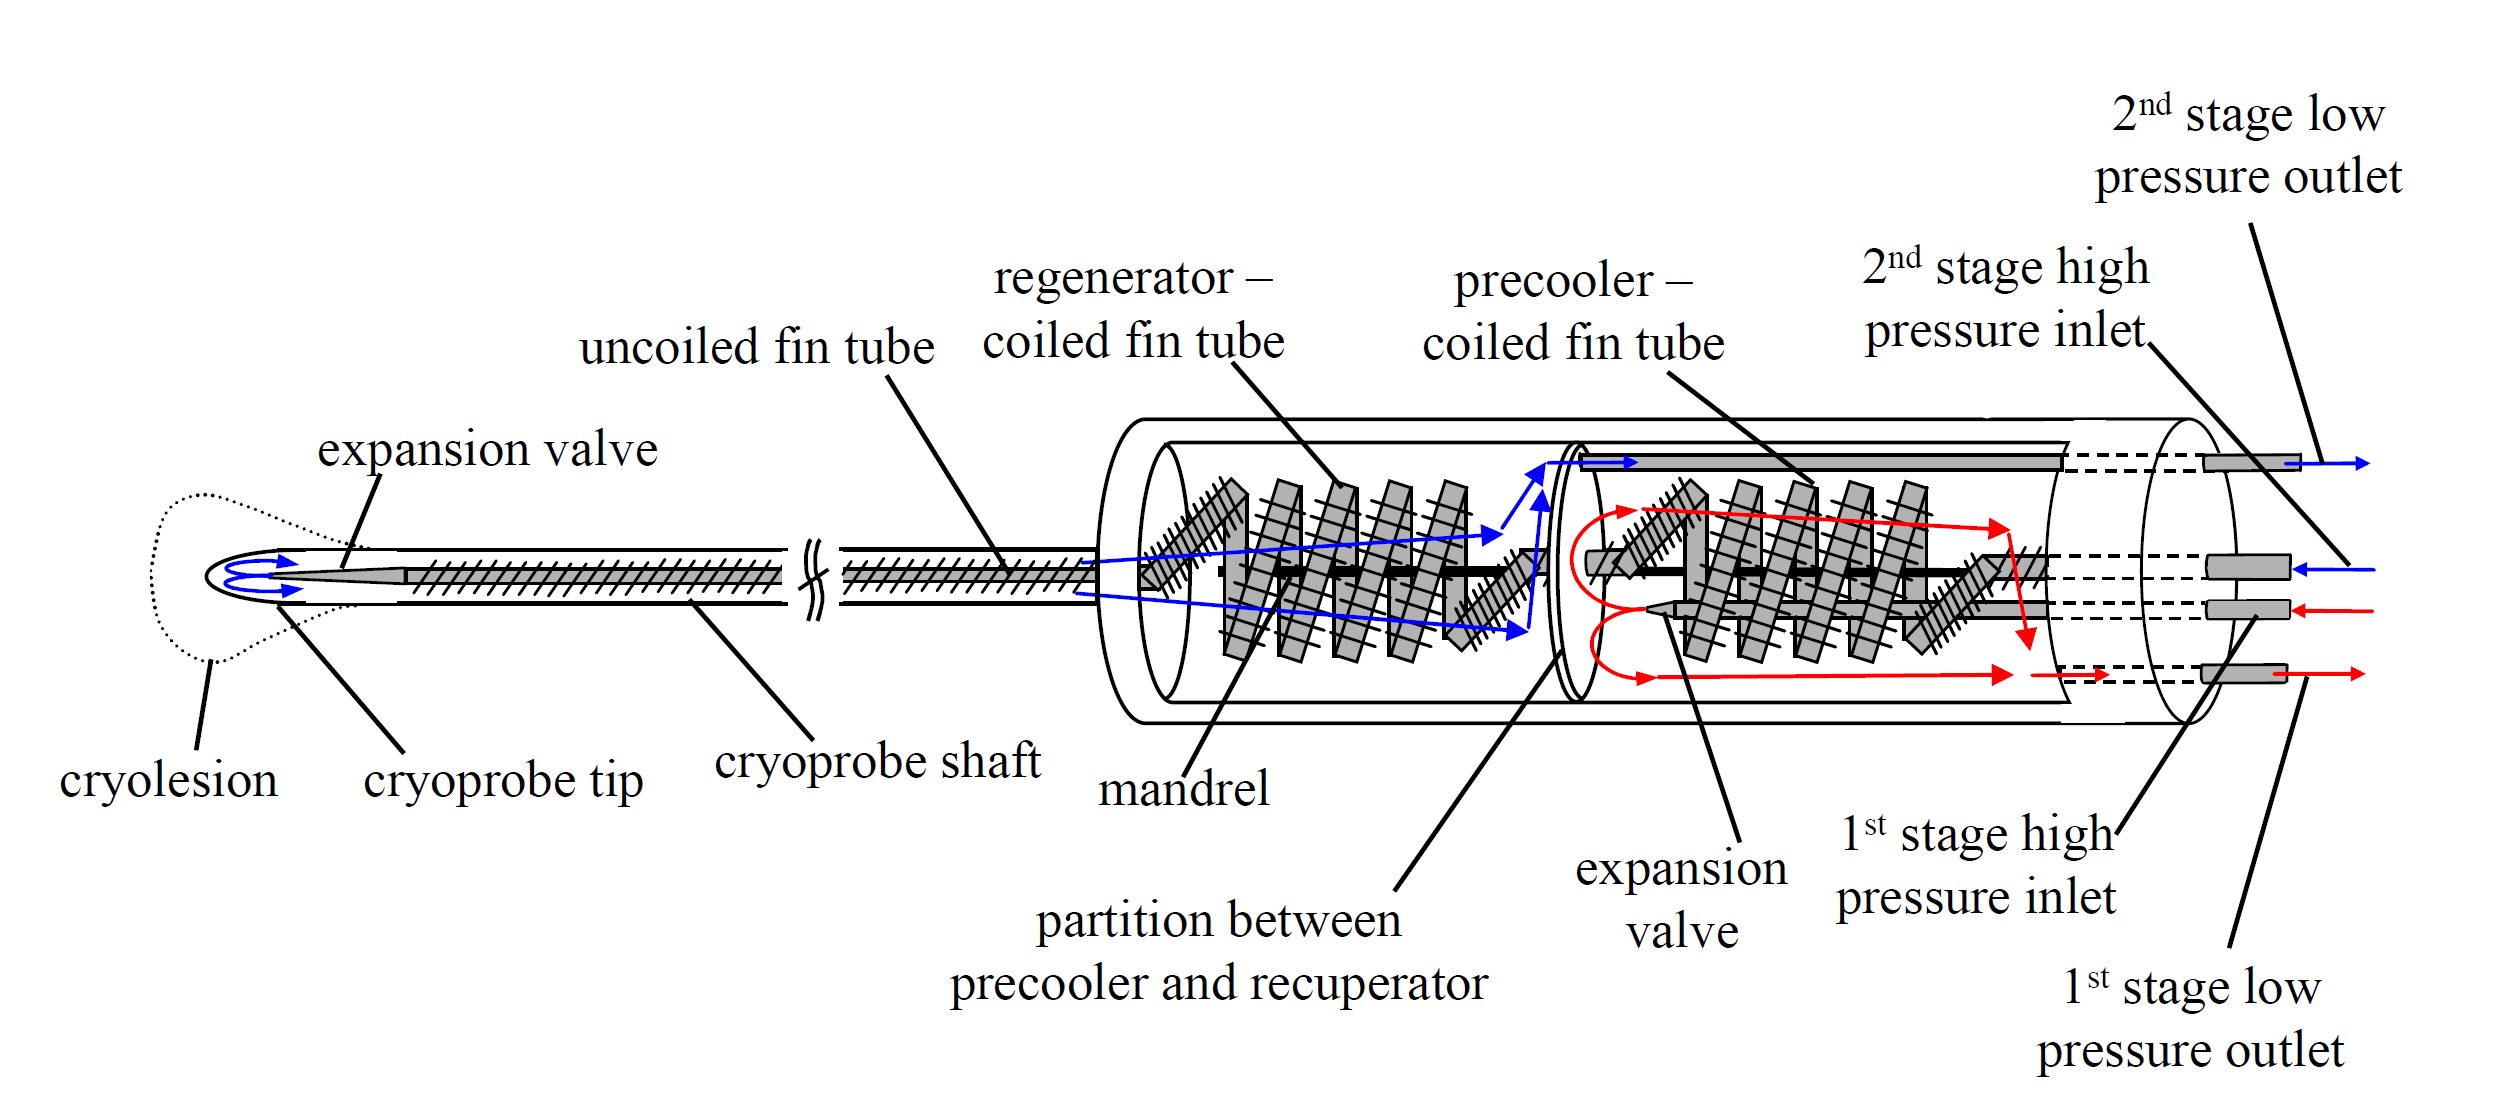
\includegraphics[width=\linewidth]{pics/1.jpg}
	\caption{...示意图\\Fig. \thefigure\quad Schematic diagram of ...}
	\label{fig:1}
\end{figure}

图\ref{fig:1}为...的示意图

\begin{table}[H]
\centering
\caption{...上的结果\\
Table \thetable\quad Results of ... on ...}
\label{tab:result}
\begin{tabular}{ccccc}
\toprule
order & 指标1 & 指标2 & 指标3 & 指标4 \\
\midrule
1 & 8\% & 1\% & 6\% & 0\% \\
2 & 8\% & 1\% & 7\% & 0\% \\
3 & 8\% & 1\% & 5\% & 0\% \\
4 & 8\% & 1\% & 6\% & 0\% \\
Average & 8\% & 1\% & 6\% & 0\% \\
\bottomrule
\end{tabular}
\end{table}

表\ref{tab:result}为...上的结果。

无监督学习是...的\cite{doersch2015unsupervised}